% Chapter4
\chapter{Implementierung} \label{chapter:thevetestcase}
\section{Modellierung der Anlage}
\section{Aufbau der Anlage}
\section{Phasen und Rezepte}
\section{HMI}
Für dieses Projekt wurde als SCADA System die Software zenon vorgegeben, daher wurde das HMI in zenon Supervisor (zenons HMI Programm) umgesetzt.\\
\\
\textbf{Visualisierung}\\
Als Ausgangspunkt für die Anlage wurde das RI-Fließeschema zur Hand genommen. Von diesem wurde die Anzahl der Elemente und die Grundstruktur übernommen. Als nächsten Schritt musste evaluiert werden, welche Inhalte des RI-Fließschemas für die Visualisierung relevant, bzw. welche Informationen/Elemente nicht vorhanden waren.
\begin{description}
\item[Wichtige Elemente]~\par
	\begin{itemize}
		\item Rohre in Verwendung kennzeichnen
		\item Sensorwerte anzeigen
		\item ....ADD MORE
	\end{itemize}
\end{description}
ABBILDUNG\\

\textbf{Einbinden von Sensorwerten}\\
Um eine Visualisierung mit aktuellen Sensorwerten zu befüllen, wird eine Verbindung zur SPS benötigt. In zenon wird eine Verbindung über zenon Logic (im weiteren nur noch Logic genannt) hergestellt.\\
\\
Als ersten Schritt, um in Logic eine SPS hinzuzufügen, musste im Unterpunkt "Feldbuskonfiguration" die Treibersoftware für die ADAM5550 SPS hinzugefügt werden. Darauf hin wurden alle Module, die an der SPS angebracht wurden, in dieser Konfiguration hinzugefügt.\\
\begin{figure}[h!]
  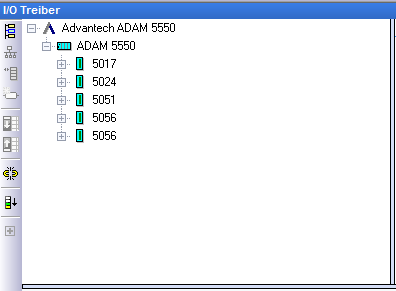
\includegraphics{graphics/implementation/Feldbuskonfiguration}
  \caption{Feldbuskonfig}%todo Grafik name
\end{figure}

Feldbuskonfiguration -> Konfiguration einfügen (Advantech ADAM 5550) -> Master/Port hinzufügen (ADAM 5550) -> Slave/Datenblock einfügen (Slot:Steckplatz an SPS; Module: Analog/Digital|In/Out|4/8/16 Channels...) -> Variable hinzufügen (Channel; Variablenname)

Variable -> Globale Variable hinzufügen (erzeugt Variable in logic und auch im supervisor zugänglich für die Visualisierung) -> In Visualisierung zu den Elemente die richtigen Variablen hinzufügen -> Bei Feldbbuskonfiguration bei richtiger I/O auf richtigem Channel hinzufügen

TEST -> logic Programm hochladen -> Variablen in logic zeigen aktuelle werte an -> check mit werten direkt von der SPS


Umrechnen von Sensorwerten: 
Durchflusssensor Digital -> etwa 900 ticks pro Liter -> Timer bid 900 ticks -> Liter/min
Füllstandsensor 4-20mA -> 4=voll, 20=leer -> Variablen/Tank Konfiguration -> Umrechnung 4=100, 20=0
Ventilstatus 0/1 -> Variablen Konfiguration -> Extremwerte farblich markieren -> Ventil Elementfarbe nach Variablen Farbe
\\
\textbf{Steuerung}\\

\textbf{Rezepterstellung}\\


\section{Ontology}
\section{Aktivitätsdiagramm}
\section{Codegenerierung}

TODO